\chapter{Rumore nei sistemi lineari}

\begin{figure}[h]
    \centering
    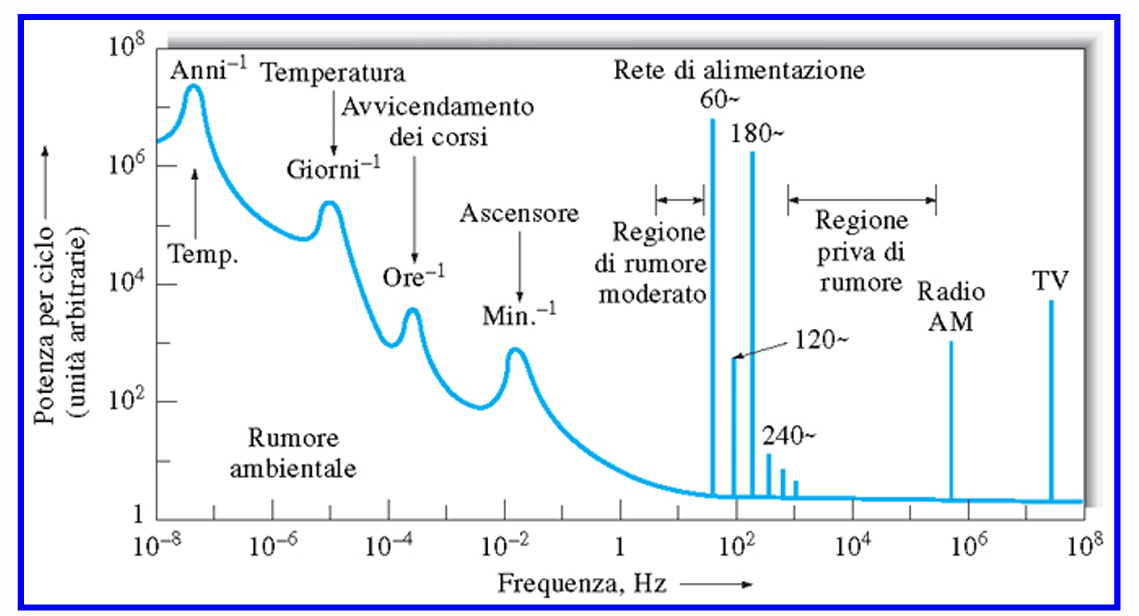
\includegraphics[scale = 0.8]{Rumore in base alla frequenza.PNG}
\end{figure}

\newpage 

\section{Banda equivalente di rumore}
\footnote{Slide del prof | Parametri di rumore sistema lineare | pag 1 \\  
Appunti di Damiano| pag 1} 

Dato un sistema lineare: 

\begin{figure}[h]
    \centering
    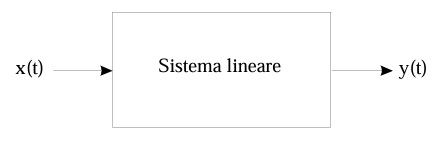
\includegraphics[scale = 1]{Blocco sistema lineare.PNG}
\end{figure}

dove x(t) è il segnale di ingresso e y(t) è il segnale di uscita dal sistema lineare, 
dal corso di Teoria dei Segnali, è noto che una generica rete 2-porte, anche contenente elementi attivi, 
è responsabile dell'introduzione di un contributo di rumore termico, 
che si sovrappone al segnale utile (i.e. segnale di ingresso) e ne degrada le caratteristiche. \newline 

\begin{tcolorbox}
    Un breve ripasso da Tds: \\
    \url{https://github.com/ciccio25/appunti-teoria-dei-segnali/blob/main/Appunti%20Teoria%20dei%20segnali.pdf} \\
    Capitolo 5 - Sistemi lineari - pag 41
\end{tcolorbox}

Allo stesso tempo, un rumore termico presente all'ingresso di una rete lineare, 
viene modificato dal transito di essa, e si ritrova in uscita amplificato (o attenuato) 
oltre che, eventualmente, con una minore occupazione spettrale (determinata dalle caratteristiche filtranti della rete resistiva). \newline 

\begin{tcolorbox}
    Un sistema lineare, a differenza di un sistema non lineare, può solo togliere le componenti in frequenza dal segnale di ingresso iniziale e non ne aggiunge di nuove
\end{tcolorbox}

Questi aspetti devono essere combinati per poter analizzare come la potenza di rumore viene alternata dal passaggio attraverso un sistema lineare 
e, soprattutto, come tale potenza aumenta quando più sistemi lineari vengono posti in cascata. \newline 

Un primo concetto utile, nel contesto delineato, è quello di banda equivalente di rumore. \newline 

Una rete 2-porte lineare è caratterizzata dalla sua funzione di trasferimento H(f) . \newline 

Quando un rumore termico, con densità spettrale di potenza bilatera $\frac{\eta}{2}$ (costante sia per le frequenze positive che per quelle negative) è applicato all'ingresso della H(f), 
la potenza di rumore in uscita sarà data da: 

{
    \Large 
    \begin{equation}
        \begin{split}
            <n^{2}>
            &= 
            \int_{-\infty}^{+\infty}
            p_{n_h}(f) 
            df
            \\
            &= 
            \int_{-\infty}^{+\infty}
            p_h(f) \cdot p_n(f) 
            df
            \\
            &= 
            \int_{-\infty}^{+\infty}
            \abs{H(f)}^{2} \cdot \abs{N(f)}^{2}
            df
            \\
            &= 
            \int_{-\infty}^{+\infty}
            \abs{H(f)}^{2} \cdot \frac{\eta}{2}
            df
            \\
            &=
            \frac{\eta}{2}
             \int_{-\infty}^{+\infty}
            \abs{H(f)}^{2} 
            df
        \end{split}
    \end{equation}
}

dove: 

\begin{itemize}
    \item $p_{n_h}(f)$ si intende la potenza del rumore (noise dall'inglese) dopo il sistema lineare 
    \item $p_h (f)$ si intende la potenza del sistema lineare 
    \item $p_n (f)$ si intende la potenza del rumore 
\end{itemize}  

\newpage 

\begin{tcolorbox}
    Per ripassare i sistemi lineari \newline 

    Da \url{https://github.com/ciccio25/appunti-teoria-dei-segnali/blob/main/Appunti%20Teoria%20dei%20segnali.pdf} \\
    Capitolo 5.2 Densità spettrale di energia e di potenza di un filtro | pag 44 \newline 

Dato x(t) il segnale di ingresso e y(t) il segnale di uscita di un sistema lineare, 
possiamo definire le loro rappresentazioni in Fourier come $X(\omega)$ e $Y(\omega)$. \newline 

Essendo: 

{
    \Large 
    \begin{equation}
        Y(\omega) = H(\omega) X(\omega)
    \end{equation}
}

le densità spettrali di energia (ove applicabili) dei segnali in ingresso e in uscita sono tra 
loro legate dalla seguente relazione: 

{
    \Large 
    \begin{equation}
        \abs{Y(\omega)} ^{2} 
        = 
        \abs{H(\omega) X(\omega)} ^{2} 
        = 
        \abs{H(\omega)} ^{2} \cdot \abs{X(\omega)} ^{2}
    \end{equation}
}

Una relazione analoga vale per gli spettri di potenza, indicati con $p_x (\omega)$ 
(per l'ingresso) e $p_y (\omega)$ (per l'uscita): 

{
    \Large 
    \begin{equation}
        p_y (\omega) = \abs{H(\omega)} ^{2} p_x (\omega)
    \end{equation}
}

$\blacksquare$ \newline 

Dunque, la densità in uscita si ottiene moltiplicando la densità in ingresso 
per il modulo al quadrato della funzione di trasferimento. \newline 


    Per ripassare il rumore \newline 

    Da \url{https://github.com/ciccio25/appunti-teoria-dei-segnali/blob/main/Appunti%20Teoria%20dei%20segnali.pdf} \\
    Capitolo 14.1 Un esempio di processo stocastico: il rumore termico | pag 162 - 163 \newline 

    Ponendo T come il valore della temperatura assoluta a cui si trova il sistema lineare in kelvin, 
    dove la relazione tra temperatura espressa in kelvin e gradi celsius è la seguente: 

    {
        \Large 
        \begin{equation}
            0\text{ }K = -273.15 \text{ } ^{\circ} C
        \end{equation}
    }


    Sapendo che: 

{
    \Large 
    \begin{equation}
        K = 1.38 \cdot 10^{-23} \frac{J}{^{\circ} K}
    \end{equation}
}

è la costante di Boltzmann. \newline 

Sapendo che il rumore è un processo "stocastico", possiamo esprimere la potenza del rumore indipendente dal tempo come: 

{
    \Large 
    
        \begin{equation}
                <P_n>
                = 
                KTB
        \end{equation}
    
}

dove $P_n$ è la "potenza disponibile". \newline 

La densità spettrale di potenza sarà: 

{
    \Large 
    \begin{equation}
        \begin{split}
        p_n(f) 
        &= 
        \frac{KT}{2}
        \\
        &= \frac{\eta}{2}
        \end{split}
    \end{equation}
}

\end{tcolorbox}

L'espressione: 

{
    \Large 
    \begin{equation}
        <n^{2}>
        =
            \frac{\eta}{2}
             \int_{-\infty}^{+\infty}
            \abs{H(f)}^{2} 
            df
    \end{equation}
}

mette in evidenza che, una volta assegnato il valore di $\frac{\eta}{2}$, 
la potenza di rumore in uscita dipende solo dall'andamento della funzione di trasferimento del sistema lineare. \newline 

Sapendo che: 

{
    \Large 
    \begin{equation}
        \frac{1}{2} \int_{-\infty}^{+\infty} \abs{H(f)}^{2} df = \abs{H_0}^{2} B_N
    \end{equation}
}

dove: 

\begin{itemize}
    \item $\abs{H_0}$ è l'ampiezza del sistema lineare 
    \item $B_N$ è la banda del rumore di ingresso al sistema lineare
\end{itemize}

Isolando $B_N$ dalla formula precedente, con dei semplici passaggi algebrici: 

{
    \Large 
    \begin{equation}
        \begin{split}
            \frac{1}{2} \int_{-\infty}^{+\infty} \abs{H(f)}^{2} df 
            &= 
            \abs{H_0}^{2} B_N
            \\
            &\updownarrow
            \\
            B_N 
            &= 
            \frac{1}{2 \abs{H_0}^{2} } \int_{-\infty}^{+\infty} \abs{H(f)}^{2} df
        \end{split}
    \end{equation}
}

Grazie alla relazione di $B_N$, possiamo riscrivere la potenza del segnale di rumore come: 

{
    \Large 
    \begin{equation}
        \begin{split}
        <n^{2}>
        &=
            \frac{\eta}{2}
             \int_{-\infty}^{+\infty}
            \abs{H(f)}^{2} 
            df 
        \\
        &= 
        \eta \frac{1}{2}
           \int_{-\infty}^{+\infty}
            \abs{H(f)}^{2} 
            df 
        \\
        &= 
        \eta \abs{H_0}^{2} B_N
        \\
        &= 
        \abs{H_0}^{2} \eta  B_N
        \end{split}
    \end{equation}
}

$\abs{H_0}^{2}$, in questa relazione di $<n^{2}>$, ha il significato di guadagno in potenza, 
che possiamo esprime anche come guadagno disponibile $G_d$ della rete 2-porte. \newline 

$B_N$ prende il nome di "banda equivalente di rumore" della rete 2-porte. \newline 

$B_N$ rappresenta la larghezza di banda di un sistema lineare con funzione di trasferimento costante e pari a $\abs{H_0}$, 
che fornisce in uscita la stessa potenza di rumore che si ha in uscita da H(f). \newline 

Dal punto di vista della potenza di rumore in uscita, i due sistemi sono perfettamente equivalenti. \newline 

\newpage 

\subsection{Osservazioni riguardo la Banda equivalente di rumore}
\footnote{Slide del prof | Parametri di rumore sistema lineare | pag 1 - 2\\  
Appunti di Damiano| pag 1 - 2} 

D'altro canto, per un dato sistema, l'integrale della formula di $B_N$: 

{
    \Large 
    \begin{equation}
        B_N 
            = 
            \frac{1}{2 \abs{H_0}^{2} } \int_{-\infty}^{+\infty} \abs{H(f)}^{2} df
    \end{equation}
}

può essere calcolato una volta 
e può essere utilizzato ai fini della valutazione della potenza di rumore in uscita: 

{
    \Large 
    \begin{equation}
        <n^{2}>
        = 
        \abs{H_0}^{2} \eta  B_N
    \end{equation}
}

Quindi passeremo da un complicato integrale da svolgere: 

{
    \Large 
    \begin{equation}
        <n^{2}>
        =
            \frac{\eta}{2}
             \int_{-\infty}^{+\infty}
            \abs{H(f)}^{2} 
            df
    \end{equation}
}

a una semplice moltiplicazione. \newline 

In effetti, il valore di $B_N$ viene normalmente specificato insieme alle altre caratteristiche del sistema, 
o comunque predeterminato per uno specifico servizio. \newline 

Ad esempio, nel caso di un segnale televisivo analogico, la banda equivalente di rumore del ricevitore può essere posta uguale a 5 MHz, 
vale a dire la massima frequenza del segnale modulante in banda base. \newline 

La conoscenza della relazione tra potenza del rumore dopo un sistema lineare $<n^{2}>$ e $B_N$, 
consente di semplificare il calcolo della potenza di rumore in uscita da una rete 2-porte quando il rumore in ingresso è a spettro piatto. \newline 

Notando un grafico di esempio riguardo alla valutazione della banda equivalente di rumore, per un generico andamento di H(f): 

\begin{figure}[h]
    \centering
    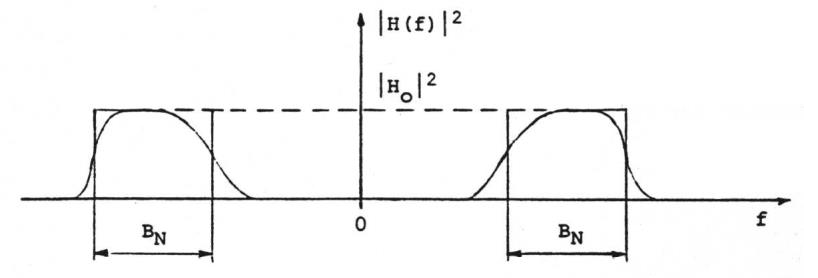
\includegraphics[scale = 1]{Valutazione della banda equivalente di rumore in un sistema.png}
\end{figure}

Se ci troviamo il caso uno spettro di rumore "colorato" come in figura (vale a dire a spettro non uniforme), 
$B_N$ non ha alcuna implicazione pratica diretta, in quanto lo spettro in uscita si ottiene dalla combinazione del modulo al quadrato della funzione di trasferimento e delle spettro di potenza in ingresso, 
ed è sempre il risultato del loro prodotto a dover essere integrato per ricavare la potenza in uscita. \newline 

In altre parole, per calcolare la potenza del rumore nel caso ideale del segnale rettangolare, abbiamo: 

{
    \Large 
    \begin{equation}
        \begin{split}
           <n^{2}>
           &=
           \frac{\eta}{2}
           \cdot
           \abs{H_0}^{2}
           \cdot
           2B 
           \\
           &=
           \eta B \abs{H_0}^2
        \end{split}
    \end{equation}
}

e possiamo dire che per un determinato $B_N$, 
la partenza del sistema equivalente è uguale a quello del sistema. \newline 

\newpage

\section{Temperatura equivalente di rumore di una rete 2-porte lineare}
\footnote{Slide del prof | Parametri di rumore sistema lineare | pag 2 - 4\\  
Appunti di Damiano| pag 2 - 4} 

Si consideri ora una rete 2-porte rumorosa, al cui ingresso si connette un resistore rumoroso a temperatura $T_i$. \newline 

All'uscita della rete 2-porte, si ha il rumore di ingresso amplificato (o attenuato) ed il rumore introdotto dalla rete 2-porte rumorosa. \newline 

Le fonti di rumore interne della rete sono, di regola, incorrelate rispetto al rumore generato dal resistore connesso in ingresso (i.e. sono indipendenti ed hanno covarianza nulla). \newline 

Pertanto, la potenza di rumore disponibile all'uscita della rete è uguale alla somma delle potenze di rumore disponibile dovute dalla: 

\begin{itemize}
    \item rumorosità della rete 
    \item rumore di ingresso amplificato (o attenuato) dalla rete
\end{itemize}

La stessa considerazione vale per le densità di potenza di rumore: 

{
    \Large 
    \begin{equation}
            \frac{\eta^{'}}{2} 
            = 
            G_d \frac{\eta}{2} + \frac{\delta \eta}{2} 
    \end{equation}
}

dove: 

\begin{itemize}
    \item $\frac{\eta^{'}}{2}$ è il segnale in uscita dalla rete 2-porte rumorosa, i.e. la densità di potenza in uscita
    \item $G_d$ è il rumore generato dal sistema lineare 
    \item  $\frac{\eta}{2}$ è il segnale di ingresso con rumore 
    \item $\frac{\delta \eta}{2}$ è la densità spettrale bilatera dovuta alla rete, i.e. la densità spettrale bilatera dovuta alla rete
\end{itemize}

Sapendo che: 

{
    \Large 
    \begin{equation}
        \begin{cases}
            \eta = K \cdot T_i 
            \\
            \eta^{'} = K \cdot T_u 
        \end{cases}
    \end{equation}
}

dove: 
\begin{itemize}
    \item $T_i$ è la temperatura in ingresso dal sistema lineare 
    \item $T_u$ è la temperatura in uscita dal sistema lineare
\end{itemize}

L'equazione della densità di potenza in uscita $ \frac{\eta^{'}}{2}$ diventa: 

{
    \Large 
    \begin{equation}
        \begin{split}
        \frac{\eta^{'}}{2} 
        &= 
        G_d \frac{\eta}{2} + \frac{\delta \eta}{2}     
       \\
       &\downarrow
       \\ 
       \frac{K \cdot T_u}{2} 
        &= 
        G_d \frac{K \cdot T_i}{2} + \frac{\delta \eta}{2}   
        \\
        &= 
        \frac{1}{2} (G_d \cdot K \cdot T_i + \delta \eta)
        \\     
        K \cdot T_u
        &= 
        G_d \cdot K \cdot T_i + \delta \eta
    \end{split}
    \end{equation}
}

Sapendo che la densità spettrale alla rete $\delta \eta$ si trova ad una temperatura $T_e$, possiamo esprimerla come: 

{
    \Large 
    \begin{equation}
        \delta \eta = G_d \cdot K \cdot T_e
    \end{equation}
}

l'espressione della densità di potenza in uscita $\frac{\eta^{'}}{2}$ possiamo continuarla ancora a semplificarla come: 

{
    \Large 
    \begin{equation}
        \begin{split}
        K \cdot T_u
        &= 
        G_d \cdot K \cdot T_i + \delta \eta
        \\
        &\downarrow
        \\
        K \cdot T_u
        &= 
        G_d \cdot K \cdot T_i + G_d \cdot K \cdot T_e
        \\
        &= 
        G_d \cdot K (T_i + T_e)
    \end{split}
    \end{equation}
}

$T_e$ prende il nome di "temperatura equivalente di rumore" della rete 2-porte. \newline 

$T_e$ rappresenta l'incremento di temperatura che occorre dare al resistore connesso all'ingresso della rete 2-porte supposta non rumorosa, 
per avere all'uscita la stessa densità di potenza disponibile di rumore che si ha con il generatore (di rumore) in ingresso a temperatura $T_i$ e rete 2-porte rumorosa. \newline 

O, spiegato in un'altra maniera, usando i sistemi equivalenti, la temperatura equivalente sposta tutto il rumore nell'ingresso, azzerando il rumore del sistema lineare. \newline 

Quindi, $T_e$ è un parametro caratteristico della rete e ne quantifica in maniera semplice ed esplicita la rumorosità. \newline 

È sufficiente aumentare di $T_e$ la temperatura di rumore in ingresso per poter considerare la rete 2-porte non rumorosa, 
pur ottenendo in uscita la stessa densità di potenza (e quindi la stessa potenza) di rumore del sistema reale. \newline 

$T_u$ rappresenta la temperatura equivalente di rumore complessiva in uscita, 
e può essere utilizzata per caratterizzare una cascata di reti 2-porte. \newline 

Quando si descrive la rumorosità del singolo dispositivo, si è soliti riferirsi alla sua sezione in ingresso, assegnando quindi direttamente il valore di $T_e$. \newline 


\newpage 

\section{Cifra di rumore di una rete 2-porte lineare}
\footnote{Slide del prof | Parametri di rumore sistema lineare | pag 3 - \\  
Appunti di Damiano| pag 3 - } 

In alternativa, alla temperatura equivalente di rumore, la rumorosità introdotta da una rete 2-porte può essere assegnata specificando la cosiddetta "cifra di rumore" (o "fattore di rumore") F. \newline 


F è definita come rapporto tra la densità di potenza disponibile di rumore in uscita da una rete 2-porte rumorosa, 
al cui ingresso sia connesso un generatore di rumore a temperatura standard $T_0$: 

{
    \Large 
    \begin{equation}
        \begin{split}
            T_0 
            &= 
            290 ^{\circ} K
            \\ 
            &= 
            (290 - 273.15) ^{\circ} C 
            \\
            &= 
            16.85 ^{\circ} C
            \\
            &\approx 
            17 ^{\circ} C
        \end{split}
    \end{equation}
}


e la densità di potenza disponibile di rumore dovuta all'amplificazione del rumore immesso in ingresso dal generatore. \newline

In formula, sulla base della notazione precedente: 

{
    \Large 
    \begin{equation}
        \begin{split}
            F 
            &= 
            \frac{\left. \eta^{'} \right|_{T_i = T_0}}{G_d \cdot K \cdot T_0 }
            \\
            &= 
            \frac{\left. G_d \cdot K (T_i + T_e) \right|_{T_i = T_0}}{G_d \cdot K \cdot T_0 }
            \\
            &=
            \frac{ G_d \cdot K (T_0 + T_e) }{G_d \cdot K \cdot T_0 }
            \\
            &=
            \frac{T_0 + T_e}{T_0}
            \\
            &= 
            \frac{T_0 (1 + \frac{T_e}{T_0})}{T_0}
            \\
            &= 
            1 + \frac{T_e}{T_0}
        \end{split}
    \end{equation}
}

Generalmente, e nella vita pratica, F cifra di rumore è sempre maggiore di 1, ma a livello teorico valgono le seguenti considerazioni teoriche. \newline 

La relazione di F con $T_e$ e $T_0$: 

{
    \Large 
    \begin{equation}
        F = 1 + \frac{T_e}{T_0}
    \end{equation}
}

stabilisce un legame esplicito tra temperatura equivalente di rumore e cifra di rumore della rete 2-porte, 
a conferma dell'equivalenza "operativa" delle due funzioni. \newline

In certi casi, può essere utile esplicitare il legame inverso, cioè: 

{
    \Large 
    \begin{equation}
        \begin{split}
        F &= 1 + \frac{T_e}{T_0}
        \\
        &\downarrow
        \\
        F - 1
        &= 
        \frac{T_e}{T_0}
        \\
        T_0 (F - 1)
        &=
        T_e 
        \\
        T_e 
        &=
        T_0 (F - 1)
        \end{split}
    \end{equation}
}

D'altro canto, moltiplicando numeratore e denominatore dall'equazione di F per la banda equivalente di rumore della rete 2-porte, 
la cifra di rumore F può anche essere riscritta come: 

{
    \Large 
    \begin{equation}
        \begin{split}
           F &= 1 + \frac{T_e}{T_0} 
           \\
           &\downarrow
           \\
           F &= \frac{<n^{'^{2}}>}{G_d \cdot <n^{2}>}
        \end{split}
    \end{equation}
}


dove: 

\begin{itemize}
    \item $<n^{2}>$ è la potenza di rumore dovuta al solo resistore a temperatura $T_0$ in ingresso (che abbiamo precedentemente calcolato) 
    \item $<n^{'^{2}}>$ è la potenza di rumore totale in uscita (comprensivo del contributo dovuto alla rete 2-porte)
\end{itemize}

Grazie a questa ultima relazione di F: 

{
    \Large 
    \begin{equation}
        F = \frac{<n^{'^{2}}>}{G_d \cdot <n^{2}>}
    \end{equation}
}

la cifra di rumore F esprime il rapporto tra il rumore in uscita dal 2-porte 
e quello che si avrebbe (sempre in uscita, stante la moltiplicazione di $<n^{2}>$ per $G_d$) 
se il 2-porte fosse ideale, cioè non introducesse alcuna rumorosità aggiuntiva. \newline 

È evidente che: 

{
    \Large 
    \begin{equation}
        F \ge 1
    \end{equation}
}

e, quanto più F risulta prossimo a 1, tanto più il comportamento del sistema lineare risulta migliore ai fini della rumorosità. \newline 

Tenendo conto che un segnale utile di potenza $S_i$ in ingresso si ritrova amplificato (o attenuato) e pari a $G_d \cdot S_i$ in uscita, 
si può semplificare ulteriormente numeratore e denominatore a secondo membro della funziona di F per $S_i$, ottenendo così: 

{
    \Large 
    \begin{equation}
        \begin{split}
            F &= \frac{<n^{'^{2}}>}{G_d \cdot <n^{2}>}
            \\
            &\quad
            \\
            &= \frac{S_i \cdot <n^{'^{2}}>}{S_i \cdot G_d \cdot <n^{2}>}
            \\
            &\quad
            \\
            &= \frac{\frac{S_i}{<n^{'^{2}}>}}{\frac{S_i \cdot G_d}{<n^{2}>} }
            \\
            &\quad
            \\
            &= \frac{\left( \frac{S}{N}\right)_{i}}{\left( \frac{S}{N}\right)_{u}}
            \\
            &\quad
            \\
            &= \frac{SNR_i}{SNR_u}
        \end{split}
    \end{equation}
}

dove: 

\begin{itemize}
    \item $SNR_i$ esprime il rapporto segnale-rumore in ingresso, in presenza del solo resistore a temperatura $T_0$
    \item $SNR_u$ esprime il rapporto segnale-rumore in uscita, includendo anche la rumorosità della rete a 2-porte
\end{itemize}

In condizioni ideali, per la rete a 2-porte, questo rapporto varrebbe 1, 
poiché segnale utile e rumore in ingresso verrebbero amplificati (o attenuati) della stessa quantità $G_d$. \newline 

In condizioni reali (cioè nel caso di un rete 2-porte rumorosa) F è sempre maggiore di 1 ed esprime il peggioramento nel rapporto segnale-rumore dovuto al 2-porte. \newline 

\newpage 

\section{Cifra di rumore di una rete 2-porte lineare e temperatura equivalente di rumore generalizzata}
\footnote{Slide del prof | Parametri di rumore sistema lineare | pag 4 - 5\\  
Appunti di Damiano| pag 4 - 5} 

È opportuno precisare che la definizione di cifra di rumore e temperatura equivalente di rumore si estende anche nel caso in cui la rumorosità introdotta dal sistema lineare è 
caratterizzata da uno spettro di potenza non uniforme e il guadagno disponibile è variabile con la frequenza. \newline 

In questo caso la F dipenderà dalla frequenza f, quindi passeremo al caso costante per ogni frequenza al caso generalizzato: 

{
    \Large 
    \begin{equation}
        \begin{split}
           F &= 1 + \frac{T_e}{T_0} 
           \\
           &\downarrow
           \\
        F(f) &= 1 + \frac{\delta \eta(f)}{\eta G_d (f)}
        \end{split}
    \end{equation}
}

Analogamente, possiamo generalizzare $T_e$ per ogni frequenza f: 

{
    \Large 
    \begin{equation}
        \begin{split}
        T_e 
        &=
        T_0 (F - 1) 
        \\
        &\downarrow
        \\
        T_e (f)
        &=
        T_0 \cdot [(F(f) - 1)] 
        \end{split}
    \end{equation}
}

Nell'ottica di caratterizzare con un unico numero la rete 2-porte, anche in questa situazione più generale, 
F(f) e $T_e (f)$ possono essere mediati sulla banda passante del rete 2-porte, 
in tal modo ottenendo: 

{
    \Large 
    \begin{equation}
        \begin{split}
            \overline{F}
            &= 
            \frac{\int_{-\infty}^{+\infty} F(f) \cdot G_d (f) df}{\int_{-\infty}^{+\infty} G_d (f) df}
            \\
            &\quad
            \\
            &= 
            \frac{1}{2 \abs{H_0}^{2} B_N} \int_{-\infty}^{+\infty} F(f) \cdot G_d (f) df
        \end{split}
    \end{equation}
}

e 

{
    \Large 
    \begin{equation}
        \begin{split}
            \overline{T_e}
            &=
            \frac{\int_{-\infty}^{+ \infty} T_e (f) \cdot G_d (f) df}{\int_{-\infty}^{+ \infty} G_d (f) df} 
            \\
            &\quad
            \\
            &=
            \frac{1}{2 \abs{H_0}^{2} B_N} \int_{-\infty}^{+ \infty} T_e (f) \cdot G_d (f) df
            \\
            &\quad
            \\
            &= 
            T_0 \cdot (\overline{F} - 1)
        \end{split} 
    \end{equation}
}

Le relazioni di $\overline{F}$ e $\overline{T_e}$ sono valide se: 

{
    \Large 
    \begin{equation}
        G_d (f) = \abs{H(f)}^{2}
    \end{equation}
}

\begin{tcolorbox}
    D'ora in poi non consideriamo la dipendenza dalla frequenza dei parametri per semplicità di notazione, 
    ma bisogna ricordarci che è possibile che esista per la teoria
\end{tcolorbox}

\newpage 

\section{2-porte in cascata}
\footnote{Slide del prof | Parametri di rumore sistema lineare | pag 5 - 6\\  
Appunti di Damiano| pag 5 - 6} 

Le espressioni sin qui introdotto sono sufficienti per descrivere la rumorosità di una singola rete 2-porte. \newline 

Cosa succede quando un certo numero di reti 2-porte vengono connessi in cascata come in figura? 

\begin{figure}[h]
    \centering
    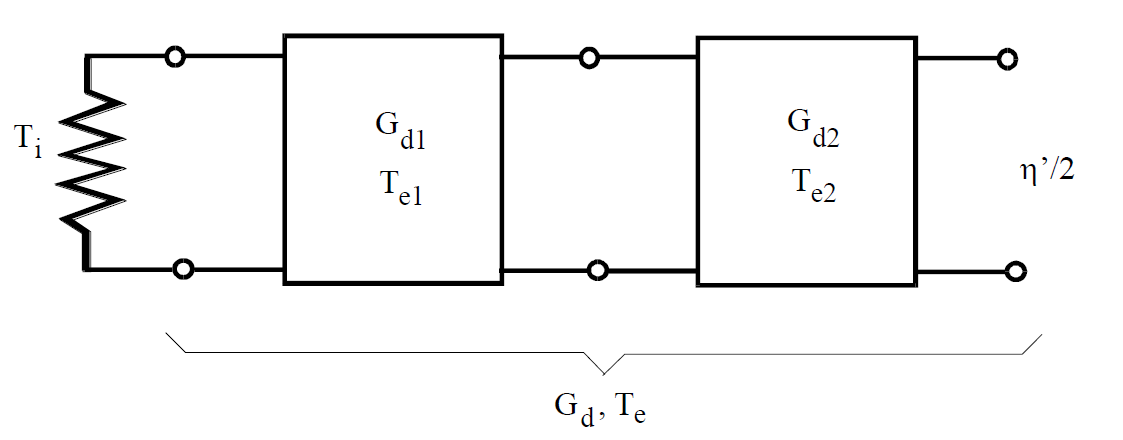
\includegraphics[scale = 0.8]{Cascata di reti 2-porte.PNG}
\end{figure}

La resistenza in ingresso, che schematizza una generica sorgente di rumore termico, si trova a temperatura $T_i$. \newline 

Ciascuna rete 2-porte è caratterizzata dal proprio guadagno disponibile, rispettivamente $G_{d1}$ e $G_{d2}$, e dalla propria temperatura equivalente di rumore, 
rispettivamente $T_{e1}$ e $T_{e2}$. \newline 

Se: 

{
    \Large 
    \begin{equation}
        G_{d1} > 1
    \end{equation}
}

la rete a 2-porte viene identificato come amplificatore. \newline 

Se: 

{
    \Large 
    \begin{equation}
        G_{d1} < 1
    \end{equation}
}

la rete a 2-porte viene identificato come attenuatrice. \newline 

Considerando solo il primo sistema lineare (quello a sinistra della figura), 
possiamo esprimere la temperatura di rumore complessiva $T_{u1}$ del primo sistema lineare 
(come studiato nelle scorse sezioni) come: 

{
    \Large 
    \begin{equation}
        \begin{split}
            K \cdot T_{u1} &= G_d \cdot K \cdot (T_i + T_{e1})
            \\
            T_{u1} &= G_d \cdot (T_i + T_{e1})
        \end{split}
    \end{equation}
}

$T_{u1}$ può essere interpretata come la temperatura equivalente in ingresso alla seconda rete 2-porte, 
in uscita dalla quale si avrà allora: 

{
    \Large 
    \begin{equation}
        \begin{split}
            T_{u2}
            &= 
            G_{d2} \cdot (T_{u1} + T_{e2})
            \\
            &= 
            G_{d2} \cdot [G_{d1} (T_i + T_{e1}) + T_{e2}]
            \\
            &=
            G_{d1} \cdot G_{d2} \cdot T_i 
            + 
            G_{d1} \cdot G_{d2} \cdot T_{e1} 
            + 
            G_{d2} \cdot T_{e2}
        \end{split}
    \end{equation}
}


Tenendo conto che il guadagno disponibile della cascata $G_d$ vale: 

{
    \Large 
    \begin{equation}
        \begin{split}
            G_d &= G_{d1} \cdot G_{d2}
            \\ 
            &\updownarrow
            \\
            G_{d2} &= \frac{G_d}{G_{d1}}
        \end{split}
    \end{equation}
}

e che, per definizione di temperatura equivalente, si deve poter scrivere: 

{
    \Large 
    \begin{equation}
        T_{u2} = G_d \cdot (T_i + T_e)
    \end{equation}
}

con $T_e$ temperatura equivalente della cascata, per confronto si ricava: 

{
    \Large 
    \begin{equation}
        \begin{split}
            T_{u2}
            &=
            G_{d1} \cdot G_{d2} \cdot T_i 
            + 
            G_{d1} \cdot G_{d2} \cdot T_{e1} 
            + 
            G_{d2} \cdot T_{e2}
            \\
            G_d \cdot (T_i + T_e)
            &=
            G_d \cdot T_i
            + 
            G_d \cdot T_{e1}
            + 
            G_{d2} \cdot T_{e2}
            \\
            G_d \cdot T_i + G_d \cdot T_e 
            &=
            \\
            G_d \cdot T_e 
            &=
            G_d \cdot T_{e1} + G_{d2} \cdot T_{e2}
            \\
            &= 
            G_d \cdot T_{e1} + \frac{G_d}{G_{d1}} \cdot T_{e2}
            \\
            &= 
            G_d \cdot (T_{e1} + \frac{T_{e2}}{G_{d1}})
            \\
            T_e
            &=
            T_{e1} + \frac{T_{e2}}{G_{d1}}
        \end{split}
    \end{equation}
}

La formula di $T_e$ appena scritta esplicita che la temperatura equivalente di due sistemi lineari in cascata 
si ottiene sommando alla temperatura equivalente del primo stadio $T_{e1}$ la temperatura equivalente del secondo stadio $T_{e2}$ per il guadagno del primo stadio $G_{d1}$. \newline 

Inoltre, la formula di $T_e$ fornisce un'altra informazione quantitativa estremamente importante: 
dovendo scegliere la collocazione relativa, ad esempio, di due stadi amplificatori, 
tendenzialmente si metterà in testa quello meno rumoroso, 
in quanto la rumorosità dell'altro stadio (maggiore) sarà ridotta del fattore $G_{d1}$. \newline 

Se il primo stadio è un attenuatore, cioè $G_{d1} < 1$, la rumorosità del secondo stadio verrebbe amplificata. \newline 

In questo caso, è meglio, se possibile, porre l'attenuatore dopo l'amplificatore. \newline 

È per questo motivo per cui il pre-amplificatore, 
per un sistema di ricezione televisivo, 
viene posto a contatto con l'antenna e prima del cavo che porta il segnale al cinescopio (la cosiddetta "discesa d'antenna"). \newline 

\newpage 

\subsection{Cifra di rumore e temperatura equivalente di rumore di una cascata di reti 2-porte lineare }
\footnote{Slide del prof | Parametri di rumore sistema lineare | pag 6 - \\  
Appunti di Damiano| pag 6 - } 

In generale, la disposizione relativa dei componenti di una cascata va ottimizzata, 
tenendo conto dei valori relativi del guadagno e della temperatura equivalente di rumore, 
in modo da minimizzare la formula di $T_e$: 

{
    \Large 
    \begin{equation}
            T_e
            =
            T_{e1} + \frac{T_{e2}}{G_{d1}}
    \end{equation}
}

La proceduta che ha consentito di ricavare la temperatura equivalente di rumore per una coppia di reti 2-porte, 
può essere estratta ad un numero n qualsiasi di sistemi lineari connessi in cascata. \newline 

La temperatura equivalente di rumore globale si ottiene dalla seguente espressione: 

{
    \Large 
    \begin{equation}
        T_e 
        = 
        T_{e1}
        + 
        \frac{T_{e2}}{G_{d1}}
        + 
        \frac{T_{e3}}{G_{d1} \cdot G_{d2}}
        + 
        \dots
        +
        \frac{T_{en}}{G_{d1} \cdot G_{d2} \cdot \dots \cdot G_{dn-1}}
    \end{equation}
}

Una eguale espressione compatta, sapendo il legame tra temperatura equivalente e cifra di rumore, si ricava come: 

{
    \Large 
    \begin{equation}
        F 
        = 
        F_{1}
        + 
        \frac{F_{2} - 1}{G_{d1}}
        + 
        \frac{F_{3} - 1}{G_{d1} \cdot G_{d2}}
        + 
        \dots
        +
        \frac{F_{n} - 1}{G_{d1} \cdot G_{d2} \cdot \dots \cdot G_{dn-1}}
    \end{equation}
}

Questa ultima formula di F è nota come "formula di Friis". \newline 

Grazie alla formula di Friis, possiamo fare le stesse considerazioni sulla cascata delle n porte partendo dalla cascata dei due sistemi lineari. \newline 

La rumorosità del primo stadio, qui espressa da $F_1$, è, in generale, la più importante nell'ambito della cascata (e va dunque adeguatamente controllata). \newline 

Si è già detto in precedenza che, uno o più stadi della cascata, possono, in realtà, presentare un comportamento da attenuatore, nel caso in cui: 

{
    \Large 
    \begin{equation}
        G_d = \frac{1}{A_d}  < 1
    \end{equation}
}

e, più che il guadagno, risulta significativo considerare l'attenuazione disponibile $A_d$, che risulta maggiore di 1. \newline 

Frequentemente, sia $G_d$ che $A_d$, sono espresse in unità logaritmiche (dB), in cui avere un numero 
in unità assolute, maggiore di 1 (o minore di 1), corrisponde a una misura in dB positiva (o negativa). \newline 

\newpage 

\section{2-porte attenuatrice: rumorosità}
\footnote{Slide del prof | Parametri di rumore sistema lineare | pag 6 - 7\\  
Appunti di Damiano| pag 6 - 7} 

È interessante chiedersi quanto valga la rumorosità di una rete 2-porte attenuatrice. \newline 

Essa è, tipicamente, realizzata utilizzando un attenuatore resistivo, 
in cui l'attenuazione è il risultato della dissipazione di potenza elettrica immensa nelle resistenze. \newline 

Dal punto di vista grafico, possiamo schematizzarlo in questa maniera: 

\begin{figure}[h]
    \centering
    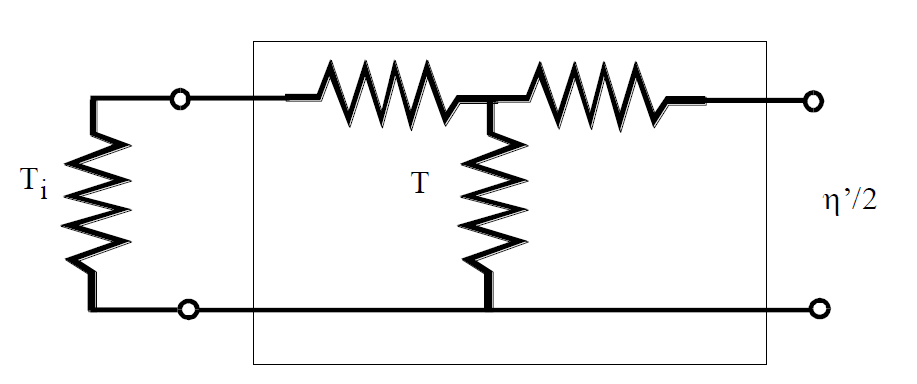
\includegraphics[scale = 0.8]{2-porte attenuatrice.PNG}
\end{figure}

Si suppone che l'attenuatore sia collegato in ingresso ad un generatore di rumore a temperatura $T_i$, 
in generale diversa dalla temperatura T dell'attenuatore. \newline 

Si può pensare che la densità di potenza disponibile nel sistema considerato sia divisa in due parti: 

\begin{itemize}
    \item la prima, pari a $K \cdot \frac{T_i - T}{2}$ è relativa all'eccesso di temperatura $T_i$ rispetto a T 
    \item la seconda, pari a $K \cdot \frac{T}{2}$ sarebbe invece, la sola densità di potenza disponibile nel caso in cui il resistore fosse alla stessa temperatura T dell'attenuatore
\end{itemize}

Se: 

{
    \Large 
    \begin{equation}
        T_i = T
    \end{equation}
}

l'insieme del resistore esterno all'attenuatore e dei resistori interni costituirebbero un'unica resistenza a temperatura T. \newline 

La densità spettrale di potenza di rumore $<P_n>$ disponibile è indipendente dal valore della resistenza. \newline  

Se si considera solo f positive, $<P_n>$ sarà uguale a: 

{
    \Large 
    \begin{equation}
        \begin{split}
            <p_n> 
            &= 
            \int_{0}^{+B} \eta(f) df 
            \\
            &= 
            K \cdot T
        \end{split}
    \end{equation}
}

Se si considera solo f positive e f negative, $<P_n>$ sarà uguale a: 

{
    \Large 
    \begin{equation}
        \begin{split}
            <p_n> 
            &= 
            \int_{-B}^{+B} \eta(f) df 
            \\
            &= 
            K \cdot \frac{T}{2}
        \end{split}
    \end{equation}
}

L'incremento di R dovuto all'attenuatore, non modificherebbe in alcun modo la rumorosità in ingresso. \newline 

Il contributo $ K \cdot \frac{T}{2}$ resta tale qualunque sia la sezione in cui si colloca (in particolare in uscita dell'attenuatore). \newline 

Il contributo $ K \cdot \frac{T_i - T}{2}$, invece, che è relativo all'eccesso di temperatura del resistore in ingresso, 
deve essere moltiplicato per il guadagno, 
ovvero, diviso per l'attenuazione disponibile. \newline 

In definitiva, la densità di potenza di rumore nella sezione di uscita vale: 

{
    \Large 
    \begin{equation}
        \begin{split}
            \frac{\eta^{'}}{2}
            &= 
            \frac{K \cdot T}{2}
            +
            \frac{K \cdot (T_i - T)}{2 \cdot A_d}
            \\
            &= 
            \frac{K \cdot T_i}{2 \cdot A_d}
            + 
            \frac{K \cdot T}{2}
            \cdot 
            \left( 1 - \frac{1}{A_d}\right)
        \end{split}
    \end{equation}
}

Indicando con $T_e$ la temperatura equivalente dell'attenuatore, 
possiamo riscrivere la densità di potenza di rumore nella sezione di uscita come: 

{
    \Large 
    \begin{equation}
        \begin{split}
            \frac{\eta^{'}}{2}
            &= 
            \frac{K \cdot (T_i - T_e)}{2 \cdot A_d}
            \\
            &= 
            \frac{K \cdot T_i}{2 \cdot A_d}
            + 
            \frac{K \cdot T_e}{2 \cdot A_d}
        \end{split}
    \end{equation}
}

Uguagliando le due formule di $\frac{\eta^{'}}{2}$ e svolgendo alcuni passi algebrici, 
possiamo ricavare $T_e$ come: 

{
    \Large 
    \begin{equation}
        T_e = T \cdot (A_d - 1)
    \end{equation}
}

Questa ultima espressione di $T_e$ esprime la temperatura equivalente di un attenuatore resistivo. \newline 

Di conseguenza, la cifra di rumore che corrisponde ad un attenuatore resistivo, vale: 

{
    \Large 
    \begin{equation}
        F = 1 + \frac{T}{T_0} \cdot (A_d - 1)
    \end{equation}
}

Nel caso particolare, ma importante, in cui l'attenuatore si trovi a temperatura standard $T_0$, 
la sua cifra di rumore uguaglia l'attenuazione disponibile, cioè: 

{
    \Large 
    \begin{equation}
        F = A_d
    \end{equation}
}

Perciò, maggiore è l'attenuazione, maggiore è la rumorosità introdotta dall'attenuatore. \newline 

Le considerazioni svolte per gli attenuatori resistivi valgono per tronchi di guida d'onda o di linee che introducono attenuazione. \newline 

\newpage

\section{Rumorosità di un sistema ricevente radio}
\footnote{Slide del prof | Parametri di rumore sistema lineare | pag 8 \\  
Appunti di Damiano| pag 8} 

Nel caso in cui si debba caratterizzare la rumorosità di un sistema ricevente per collegamenti radio, 
in cui l'insieme degli apparati che costituiscono il ricevitore (cavi, amplificatori, mixer, $\dots$) sia chiuso in ingresso dall'antenna ricevente, 
la temperatura di ingresso $T_i$ deve essere assunta la temperatura di antenna $T_A$. \newline 

La somma della temperatura equivalente del radioricevitore prende il nome di temperatura di sistema $T_S$, 
che si ottiene come: 

{
    \Large 
    \begin{equation}
        T_S = T_A + T_e
    \end{equation}
}

$T_A$ non è la temperatura fisica dell'antenna, ma dipende da dove viene puntata. \newline 

Quando $T_A \approx T_0$, $T_S$ si può esprimere come: 

{
    \Large 
    \begin{equation}
        T_S \approx T_0 \cdot F_r
    \end{equation}
}

dove $F_r$ è la cifra di rumore del ricevitore. \newline 

\newpage 

\section{Conclusioni riguardo la temperatura equivalente}
\footnote{Slide del prof | Parametri di rumore sistema lineare | pag 8\\  
Appunti di Damiano| pag 8} 

In chiusura, si vuole ribadire l'importanza applicativa della definizione di temperatura equivalente (o cifra di rumore a cui essa è legata). \newline 

Trasferendo la rumorosità dovuta alla rete 2-porte (o alla cascata di reti 2-porte) in un incremento della temperatura che schematizza la rumorosità in ingresso, 
essa consente di considerare la rete stessa non rumorosa. \newline 

Come conseguenza, il rapporto segnale-rumore è costante in qualunque sezione del sistema lineare in cui venga calcolato. \newline 

Segnale utile e rumore sono trattati allo stesso modo da blocchi ideali. \newline 

Ovviamente, ciò che resta invariato è un rapporto segnale-rumore in cui la potenza di rumore è onnicomprensiva e tiene conto, in qualunque sezione, anche della rumorosità dei blocchi posti a valle. \newline 

D'altro canto, è questa la rumorosità che interessa ai fini del dimensionamento del sistema e della valutazione delle sua prestazioni. \newline 

Una potenza di rumore che escluda alcuni contributi può essere utile per capire la dinamica del disturbo, 
ma non ha alcuna utilità della caratterizzazione del sistema complessivo. \newline 

Il rapporto segnale-rumore può essere riferito e calcolato in una qualunque sezione. \newline 

Tipicamente ci si colloca in ingresso, ma ciò non rappresenta una scelta obbligata. \newline 

Il fatto che l'SNR resti invariato nel sistema equivalente non implica che la potenza di segnale utile o quella di rumore, considerati individualmente, 
restino pure invariati. \newline 

Al contrario, la potenza S, ad esempio, viene moltiplicata, nel passaggio dall'ingresso all'uscita, per il guadagno disponibile $G_d$, 
lo stesso si verifica per la potenza di rumore. \newline 

Di conseguenza, anche la temperatura equivalente della cascata (cui la potenza di rumore risulta proporzionale) 
può essere riportata in una qualunque sezione, 
semplicemente moltiplicando o dividendo per gli opportuni guadagni (dei blocchi che separano le sezioni considerate). \newline 

\newpage 

\section{Da segnale analogico a segnale digitale}
\footnote{Slide del prof | Parametri di rumore sistema lineare | pag 13\\  
Appunti di Damiano| pag 13} 

In un sistema analogico, le potenze di rumore introdotte dalle singole tratte, supposte tra loro indipendenti, si sommano. \newline 

La potenza di rumore, in analogico, è approssimativamente ad n volte il risultato che si ottiene considerando la tratta singola. \newline 

Ciò si traduce in una significativa degradazione del rapporto segnale-rumore il cui valore, 
è inversamente proporzionale al numero delle tratte considerate. \newline 

Il rapporto segnale rumore è il parametro di merito da utilizzare per esprimere la qualità di un segnale analogico. \newline 

La situazione è radicalmente diversa quando si considera un sistema numerico (sempre organizzato in n tratte). \newline 

Qui il parametro di merito diventa la probabilità di errore e si dimostra che (sarà dimostrato nei successivi capitoli) che, in questo caso, 
sono proprio le probabilità di errore a dover essere sommate, nella cascata di n tratte, per ottenere la probabilità di errore complessiva che influenza l'intero collegamento. \newline 

Questo risultato, peraltro, è conseguenza di una diversa organizzazione di sistema di trasmissione. \newline 

Mentre nel caso analogico i ripetitori posti alla fine di ogni tratta sono essenzialmente degli amplificatori, 
nel caso numerico può essere più conveniente effettuare ad ogni stazione intermedia una "rigenerazione" del segnale, 
cioè estrarre i dati ed effettuare una nuova trasmissione nella tratta successiva. \newline 

È proprio questa procedura che consente di evitare l'accumulazione dei disturbi. \newline 

Per fissare le idee, si può supporre che, in ciascuna tratta, la trasmissione avvenga con le modalità di un canale binario simmetrico caratterizzato da una probabilità di transizione errata 
sul simbolo binario uguale a p. \newline 

Si ha, allora, un errore finale sul simbolo trasmesso se avviene in un numero dispari di tratte: 
con un numero pari di errori: infatti, si ha una compensazione e, in uscita, si riottiene il simbolo corretto. \newline 

Ad esempio se si ha il simbolo 1, se le tratte sono pari, il simbolo ritorna a 1; 
se le tratte sono dispari, il simbolo o può essere 1 o 0, che è diverso da 1. \newline 

Ma la probabilità di errore su 3, 5, $\dots$ tratte è in genere (se p è piccola) trascurabile, 
rispetto alla probabilità di sbagliare su una sola delle n tratte. \newline 

Quest'ultima probabilità, che approssima, nel senso precisato, la probabilità di errore globale $P_{E}^{n}$ vale: 

{
    \Large 
    \begin{equation}
        \binom{n}{1}p(1-p)^{n-1} 
        \approx 
        n \cdot p 
        \approx 
        P_{E}^{(n)}
    \end{equation}
}

Questa ultima formula esplicita che la probabilità di errore si sommano nella cascare di n tratte. \newline 

Questa formula è nettamente favorevole rispetto a quella valida nel caso di sistema analogici. \newline 

In particolare, tenendo conto che la probabilità di errore decresce molto velocemente al crescere del rapporto segnale-rumore (tipicamente con legge esponenziale), 
si verifica che, aumentando anche considerevolmente il numero di tratte la variazione corrispondente nel rapporto segnale-rumore, si mantiene costante. \newline 

\newpage 

\subsection{Calcolo numerico di n tratte per un segnale analogico rispetto al segnale digitale}
\footnote{Slide del prof | Parametri di rumore sistema lineare | pag 13\\  
Appunti di Damiano| pag 13} 

Ad esempio, nel caso di un segnale analogico, considerando: 

{
    \Large 
    \begin{equation}
        n = 10
    \end{equation}
}

tratte, il rapporto segnale e rumore deve essere aumentato di 10 dB per mantenere la qualità che si avrebbe con una tratta singola. \newline 

Considerando invece un segnale numero in banda base con forma d'onda anti-podali, 
e volendo conseguire una probabilità di errore globale: 

{
    \Large 
    \begin{equation}
        P_{E}^{(n)} = 10^{-5}
    \end{equation}
}

sappiamo che, considerando $n = 1$: 

{
    \Large 
    \begin{equation}
        \binom{n}{1}p(1-p)^{n-1} 
        \approx 
        n \cdot p 
        \approx 
        P_{E}^{(n)}
    \end{equation}
}

quindi: 


{
    \Large 
    \begin{equation}
        \begin{split}
        n \cdot p 
        &\approx 
        P_{E}^{(n)} 
        \\
        &\downarrow
        \\
        1 \cdot p 
        &\approx 
        P_{E}^{(n)}
        \\
        p 
        &=
        P_{E}^{(n)}
        = 
        10^{-5} 
        \end{split} 
    \end{equation}
}

se invece $n = 10$: 

{
    \Large 
    \begin{equation}
        \begin{split}
        n \cdot p 
        &\approx 
        P_{E}^{(n)} 
        \\
        &\downarrow
        \\
        n \cdot p 
        &\approx 
        P_{E}^{(n)}
        =
        10^{-5}  
        \\
        p 
        &=
        \frac{P_{E}^{(n)}}{n}
        = 
        \frac{10^{-5}}{10}
        = 
        10^{-6}
        \end{split} 
    \end{equation}
}


Come si dimostrerà, trattando la qualità delle trasmissioni numeriche, 
in particolare per il caso di segnali antipodali, 
il rapporto segnale-rumore quando si passa da n = 1 a n = 10, 
deve essere aumentato di circa 1 dB. \newline 

Un valore significativamente minore rispetto a quanto richiesto nel caso di collegamento analogico. \newline 

\newpage 




